\section{Análise de casos de uso}
O diagrama de análise usa fronteiras, controles e entidades, sem atributos ou métodos. Representa somente o núcleo implementado até a Sprint 4: autenticação, usuários, pacientes, registros de acesso e relatórios de acesso. O vínculo ``cadastrado por'' associa cada paciente ao usuário responsável pelo cadastro, e cada registro de acesso pertence a um usuário.

\begin{sloppypar}
O UC15 usa \path|ControleRelatorios|, realizado por \path|FacadeSingletonController.generateAccessReport| e \path|AccessReportTemplate|. A fachada autoriza o Administrador antes da leitura dos acessos; o controle gera as mesmas estatísticas para HTML e CSV (RF18). As fronteiras \path|TelaRelatorios| (\path|/access-reports|) e \path|RotaRelatorios| (\path|GET /api/access-reports|) oferecem o download ao Administrador. O \path|ControleAutenticacao| registra um \path|RegistroDeAcesso| para cada credencial aceita (RF17).
\end{sloppypar}

\begin{figure}[H]\centering
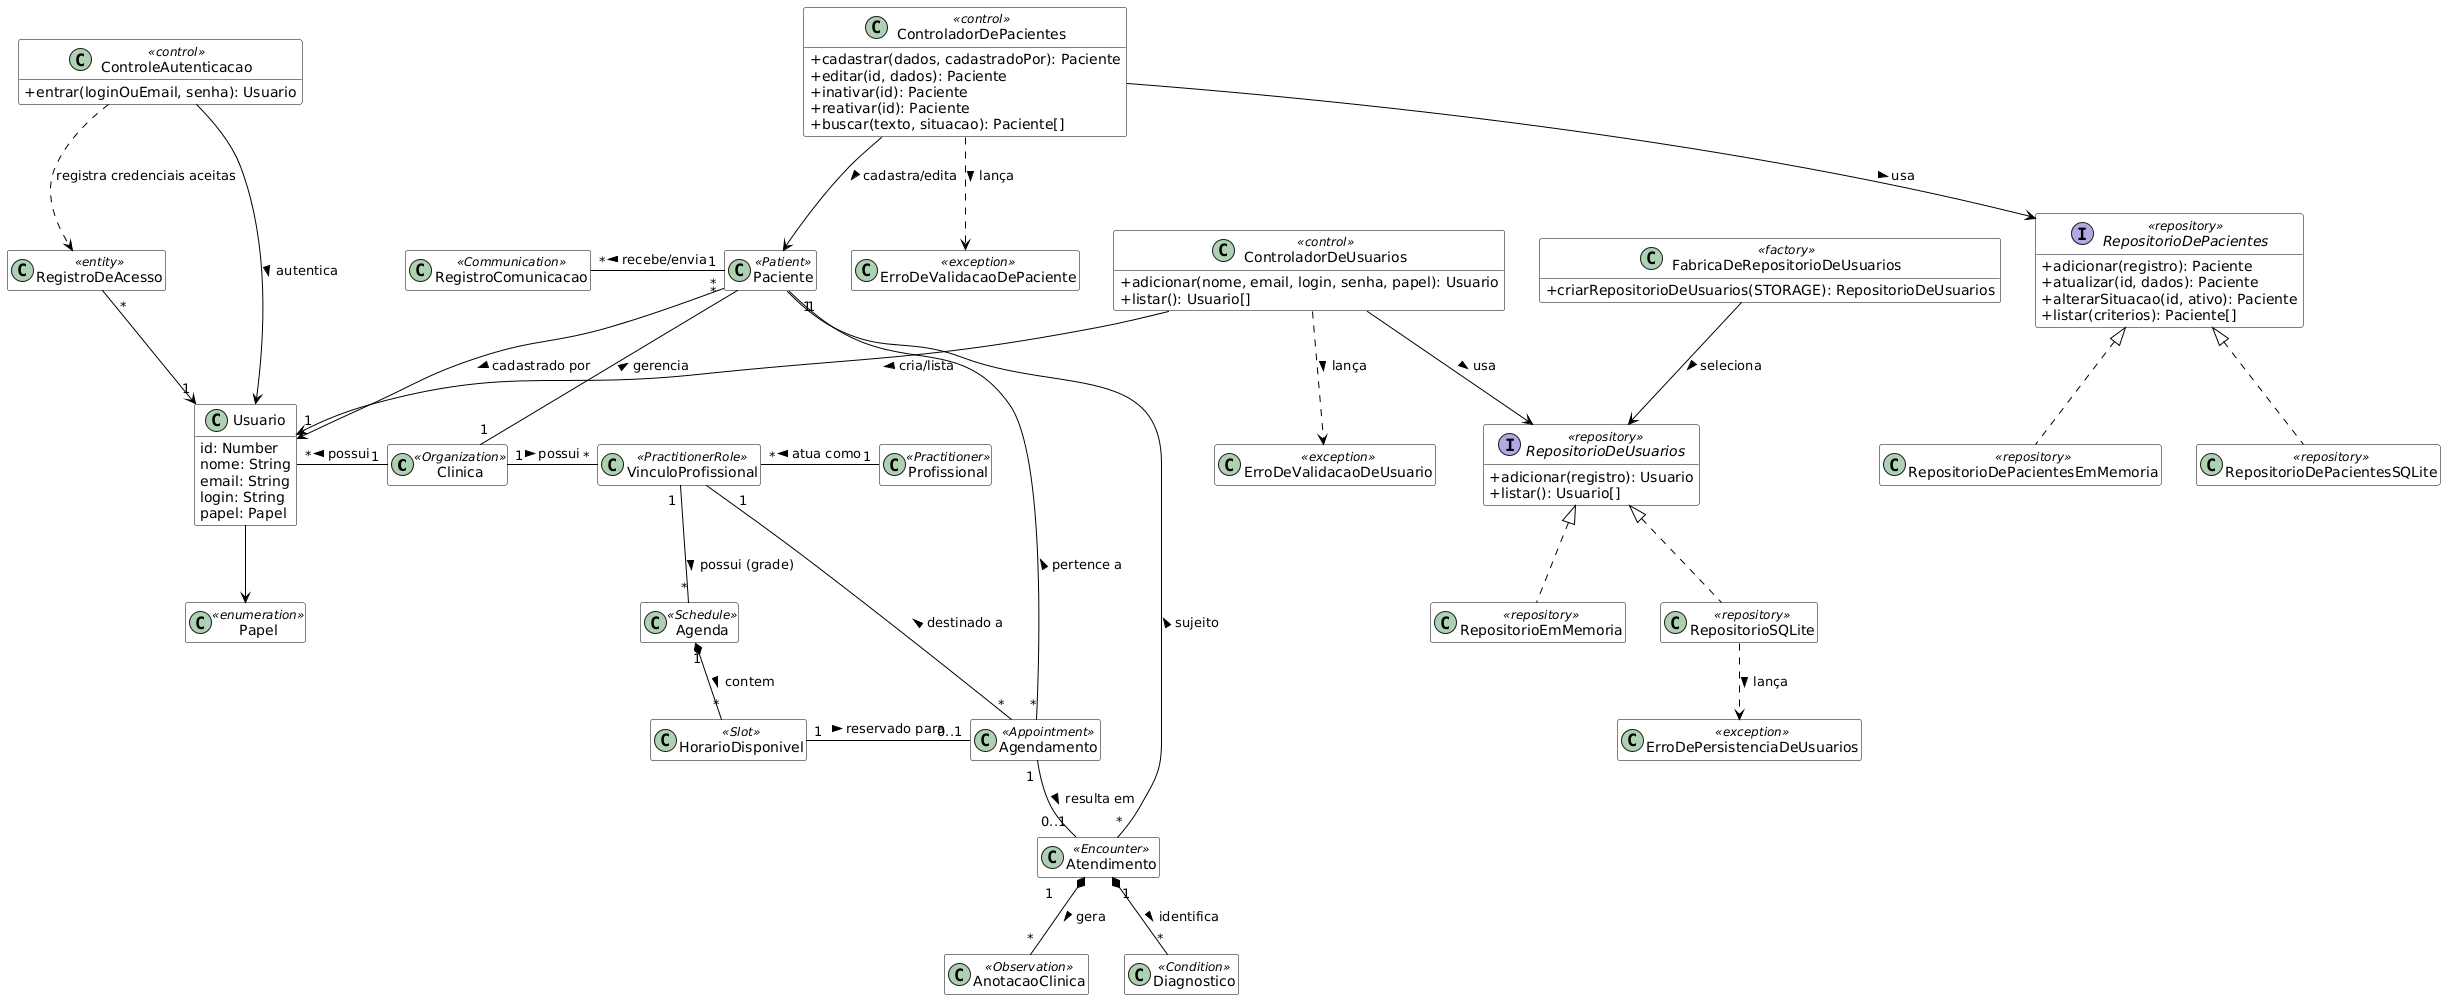
\includegraphics[width=\textwidth,height=0.8\textheight,keepaspectratio]{images/classes-de-analise.png}
\caption{Classes de análise do núcleo implementado.}
\end{figure}